%%%%%%%%%%%%%%%%%%%%%%%%%%%%%%%%%%%%%%%%%
% Frequently Asked Questions
% LaTeX Template
% Version 1.0 (22/7/13)
%
% This template has been downloaded from:
% http://www.LaTeXTemplates.com
%
% Original author:
% Adam Glesser (adamglesser@gmail.com)
%
% License:
% CC BY-NC-SA 3.0 (http://creativecommons.org/licenses/by-nc-sa/3.0/)
%
%%%%%%%%%%%%%%%%%%%%%%%%%%%%%%%%%%%%%%%%%

\documentclass[11pt]{article}

\usepackage[margin=1in]{geometry} % Required to make the margins smaller to fit more content on each page
\usepackage[linkcolor=blue]{hyperref} % Required to create hyperlinks to sections from elsewhere in the document
\hypersetup{pdfborder={0 0 0}, colorlinks=true, urlcolor=blue} % Specify a color for hyperlinks
\usepackage{microtype} % Slightly tweak font spacing for aesthetics
\usepackage[utf8]{inputenc}
\usepackage[T1]{fontenc}
\usepackage{lmodern}
\usepackage{sidecap}
\usepackage{listings,xcolor}
\usepackage{graphicx}

\setlength\parindent{0pt} % Removes all indentation from paragraphs

\ifdefined\frenchmanual
  \newcommand\mtext[2]{#1}
\else
  \newcommand\mtext[2]{#2}
\fi



\begin{document}

%----------------------------------------------------------------------------------------
%	TITLE
%----------------------------------------------------------------------------------------


\begin{flushright}
  \includegraphics[width=0.1\textwidth]{bretagne_quadri.pdf}
\end{flushright}

\begin{center}
\Huge{\bf \emph{\mtext{Wi2Me Recherche - Manuel d'utilisation}{Wi2Me Research - User Manual}}} % Main title
\end{center}

\begin{flushleft}
\mtext{Ce document présente l'utilisation de l'application de mesure Wi2Me Recherche développée par TELECOM Bretagne. Pour plus d'information ou de support :}{This Document presents the steps required to perform mesurements using the Wi2Me Research application developed by TELECOM Bretagne. For more information or support, feel free to contact : }

Tanguy Kerdoncuff \\ 
tanguy.kerdoncuff@telecom-bretagne.eu\\
+332 99 12 70 49 \\
TELECOM Bretagne - Dept. RSM\\
2, Rue de la Chataigneraie \\
35100 Cesson Sévigné\\
\end{flushleft}

%----------------------------------------------------------------------------------------
\section{\mtext{Lancer Wi2Me}{Starting Wi2Me}}\label{starting}

\begin{SCfigure}[\sidecaptionrelwidth][!h]
  \centering
  \caption{ \mtext{Lancer l'application en pressant sur l'icône Wi2Me Research du bureau.}{Start the application by pressing the Wi2Me Research application on the desktop.}}
  \includegraphics[height=0.4\textheight]{open.png}
\end{SCfigure}

\begin{SCfigure}[\sidecaptionrelwidth][!h]
  \centering
  \caption{ \mtext{Ouvrir le menu de wi2me en utilisant le button en bas à gauche (ou le bouton menu physique s'il existe).}{Open the application menu by using the menu button in the bottom left (or your phone's physical menu button if it exists).}}
  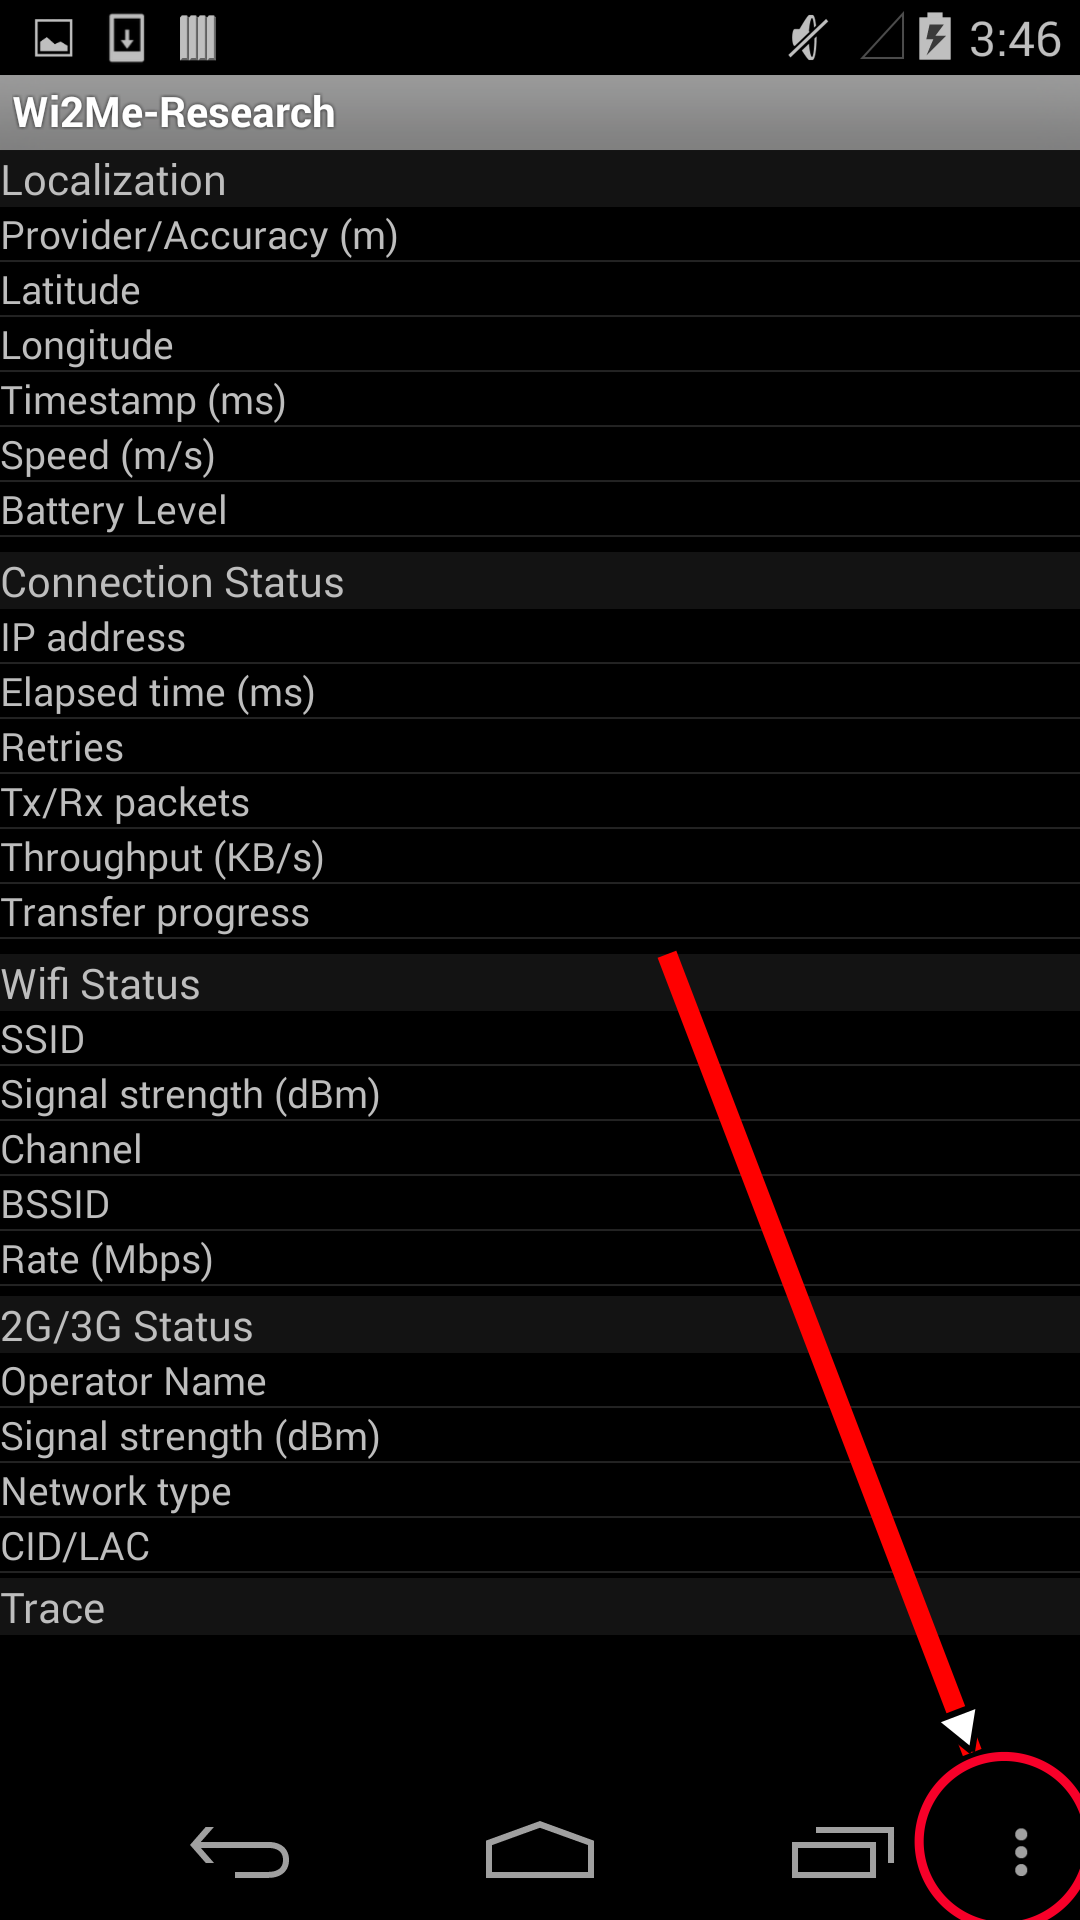
\includegraphics[height=0.4\textheight]{MenuStart.png}
\end{SCfigure}


\begin{SCfigure}[\sidecaptionrelwidth][!h]
  \centering
  \caption{\mtext{Déclencher les mesures en appuyant sur le bouton Start. Le menu va se fermer et certaines données commenceront à s'afficher à l'écran. L'écran peut maintenant être éteint.}{Trigger the mesurements by pressing the start button in the menu. The overlay menu will close and some information will start being displayed on screen. The phone's screen can now be turned off to save battery.}}
  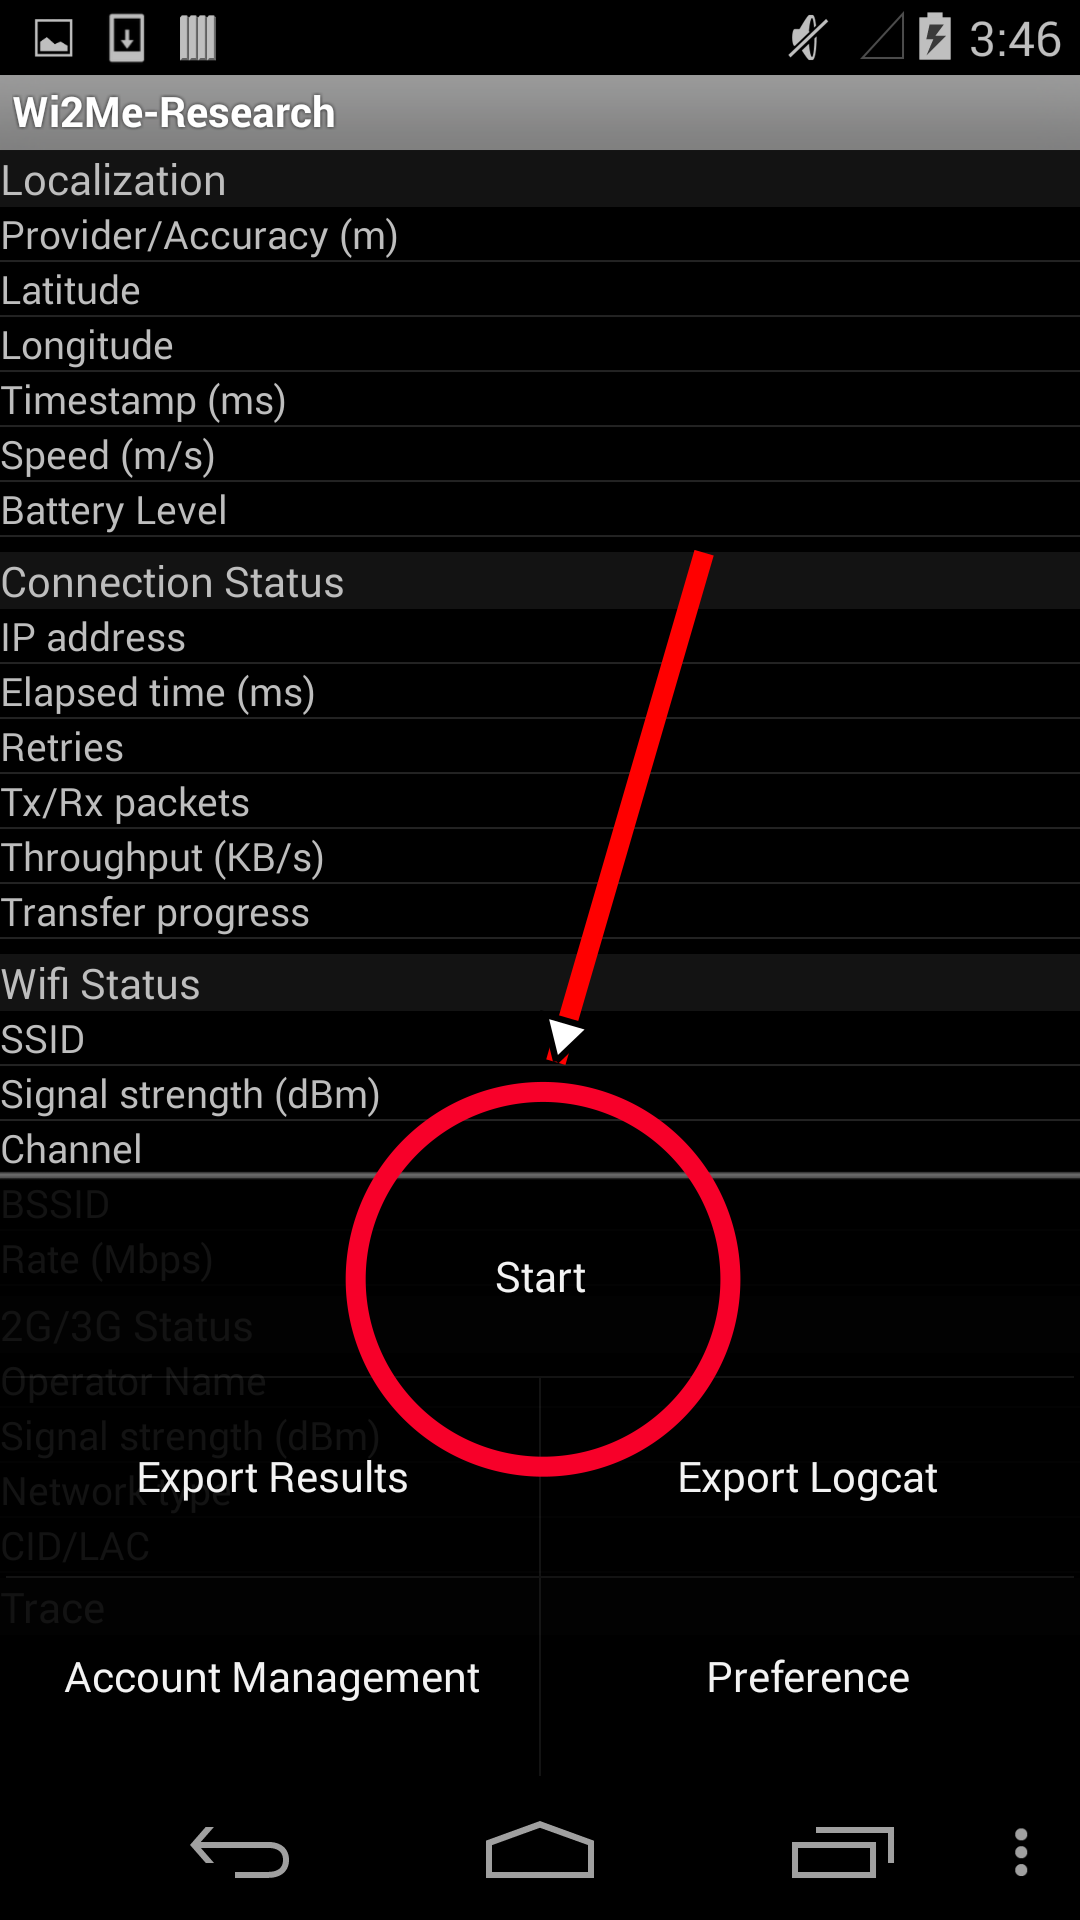
\includegraphics[height=0.4\textheight]{start.png}
\end{SCfigure}
\clearpage

%------------------------------------------------
\section{\mtext{Arrêter wi2me}{Stopping Wi2Me}}\label{stopping}

\begin{SCfigure}[\sidecaptionrelwidth][!h]
  \centering
  \caption{\mtext{ Ouvrir le menu de wi2me en utilisant le menu en bas à gauche (ou le bouton menu physique s'il existe)}{Open the application menu by using the menu button in the bottom left (or your phone's physical menu button if it exists).}}
  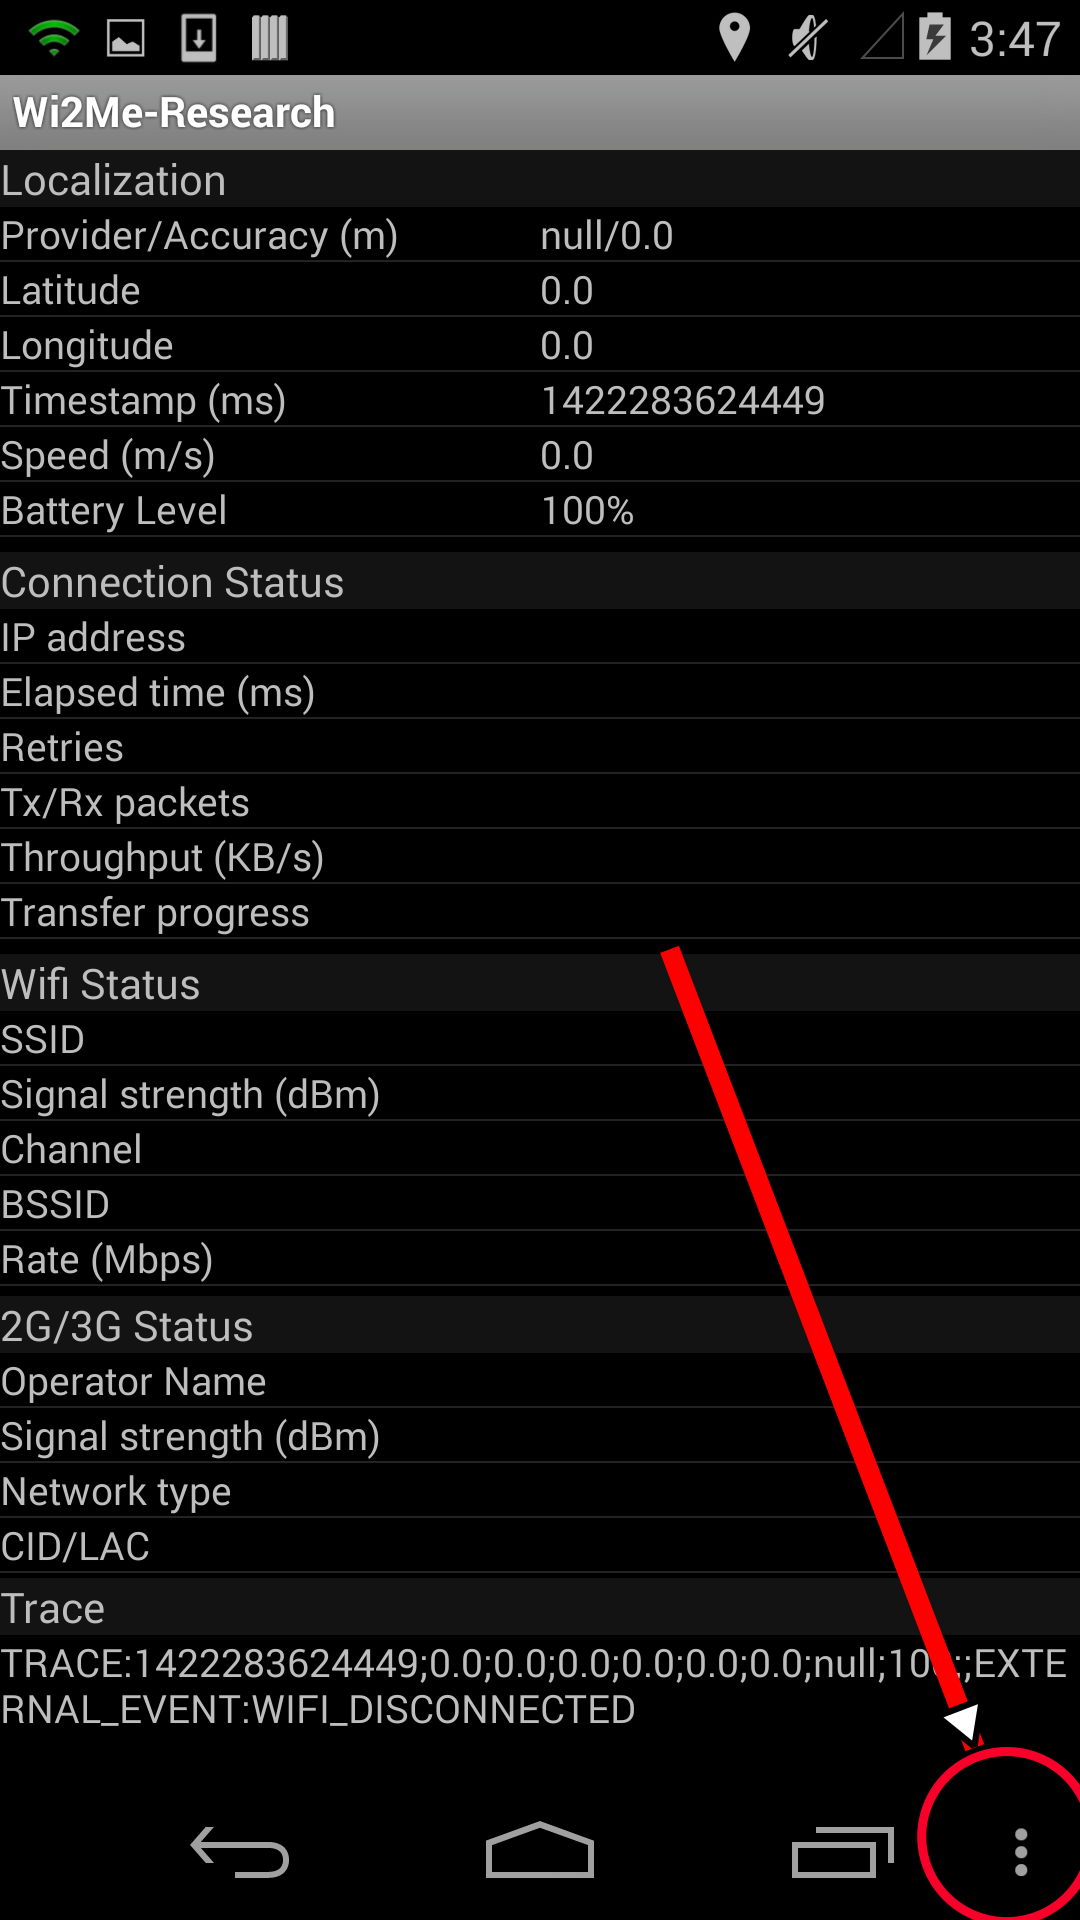
\includegraphics[height=0.4\textheight]{MenuStop.png}
\end{SCfigure}

\begin{SCfigure}[\sidecaptionrelwidth][!h]
  \centering
  \caption{\mtext{Presser le bouton stop. Après un cours moment, les données ne seront plus affichées dans l'application, qui pourra être fermée ou réduite.}{Press the stop button. After some processing, the application will stop diplaying data and can be closed or reduced.}}
  \includegraphics[height=0.4\textheight]{stop.png}
\end{SCfigure}

\newpage
\section{\mtext{Export de résultats}{exporting results}}\label{sec:exporting}


\begin{SCfigure}[\sidecaptionrelwidth][!h]
  \centering
  \caption{
\mtext{Après une session de mesure, il faut les exporter dans un format
générique. Pour cela, ouvrir le menu et choisir l'entrée 'export results'. Un
popup s'ouvre alors, y choisir 'Export to SD'. Cela crée un fichier sur la carte
SD du téléphone, nommé trace\_XXXX\_YYYY ou YYYY est un timestamp, et XXXX un
identifiant du téléphone.}{After a data gathering phase, you will need to export your results for further processing. To do so, open the menu again, and press the 'export results' button. A pop up will appear asking the type of export you wish to use. Select the "Export to" SD option.
Once this is done, you can find your measurements at the phone's sdcard root,
under the name TraceLog\_XXXX\_YYYY where XXXX is an identifier unique to the
phone, and YYYY, a timestamp of the moment you performed the export.
}
}
  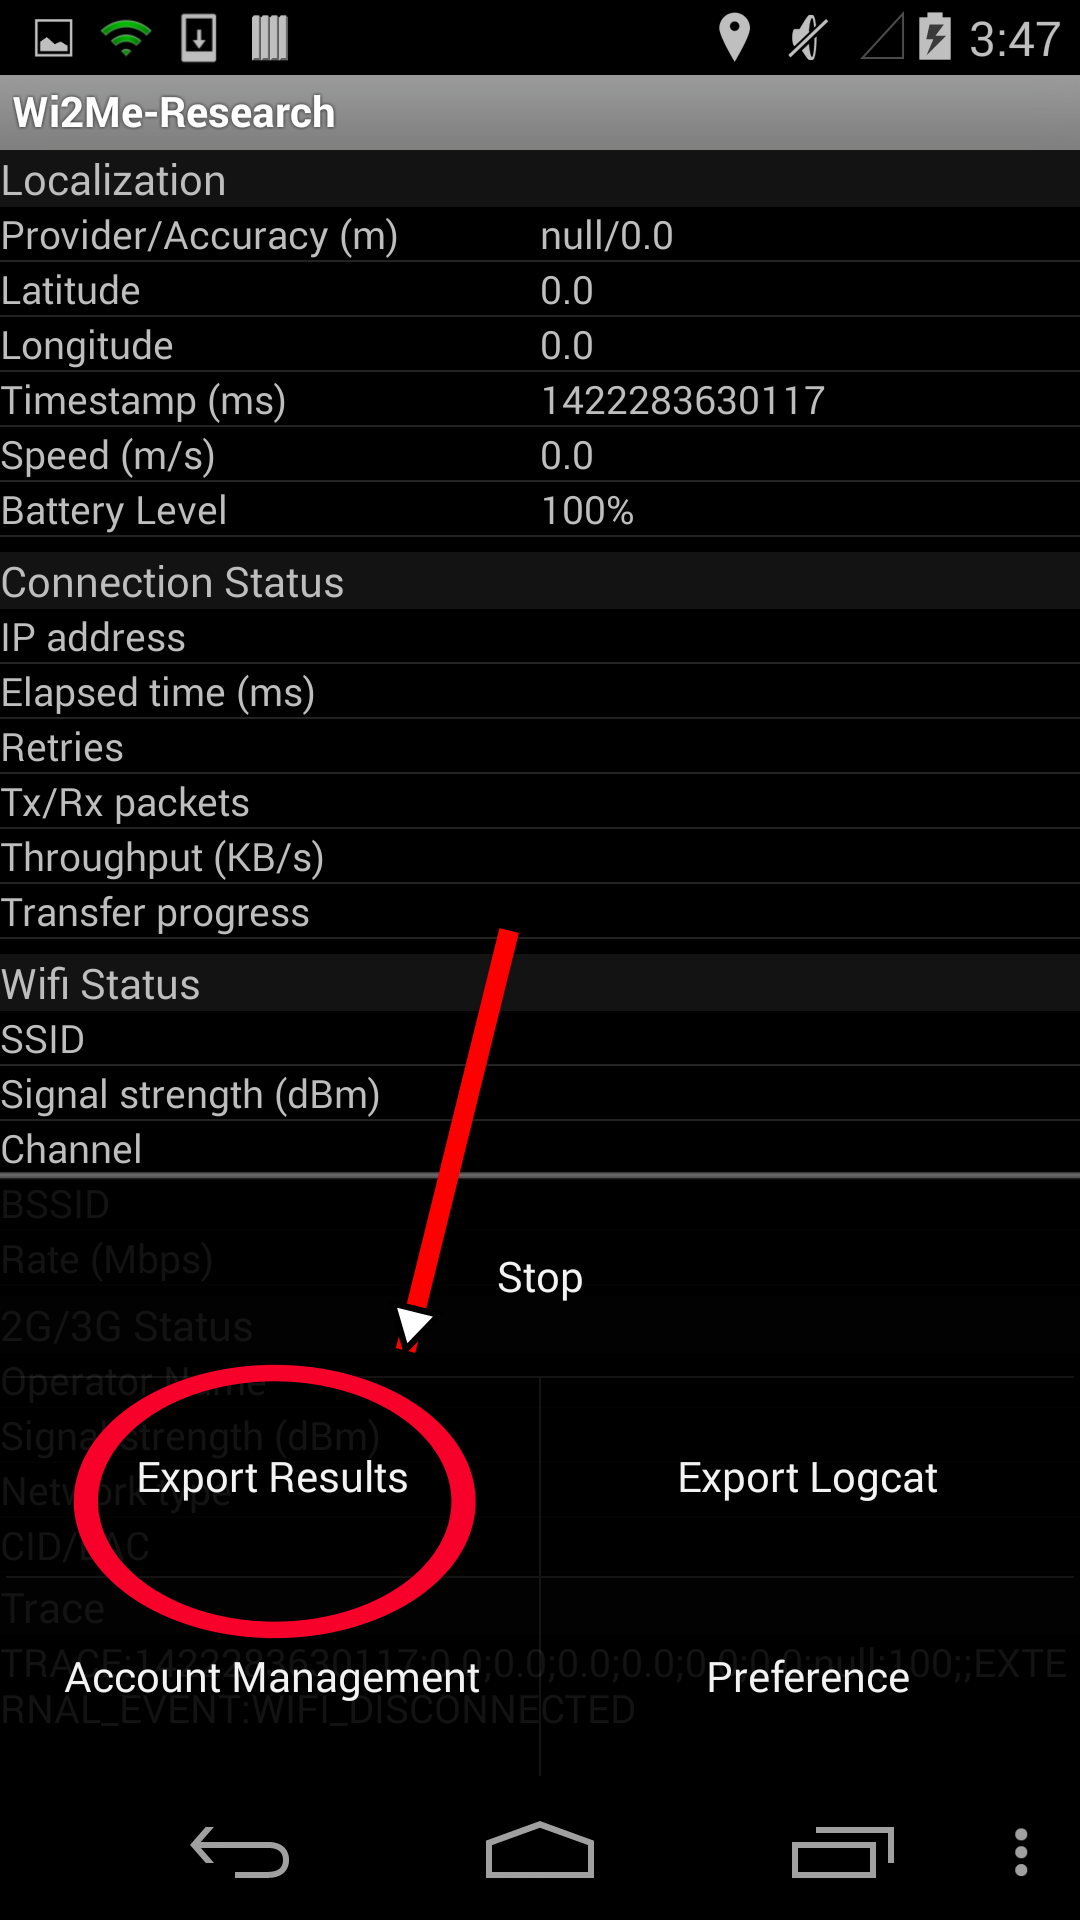
\includegraphics[height=0.4\textheight]{export.png}
\end{SCfigure}

\newpage

\section{\mtext{Configurations Wi2Me}{Wi2Me Configurations}}\label{sec:jsonconf}

\mtext{Wi2Me a une architecture modulaire, et peut fonctionner en exécutant
plusieurs variétés de taches, dont certaines sont paramêtrables. Ces taches sont
définies dans des fichiers json livrés avec l'application. Pour choisir ces
fichiers, presser sur l'entrée 'COMMAND\_FILE' des préférences de l'application.
Un explorateur s'ouvrira.  Naviguer à /sdcard/Wi2MeRecherche/configs et choisir
l'un des fichiers.

Les configurations  disponibles sont :
\begin{itemize}
\item ble.json : Interaction par BLE avec un objet Pycom Lopy, écriture des
coordonnées GPS, lecture d'vènements
\item defconf.json : configuration par défaut (legacy), scan et connection
wifi/cellulaire, transfert de fichier
\item emulated\_connections.json : configuration d'émulations de connections
wifi par scans manuels monofréquence, requiers un téléphone rooté et un binaire
de iw.
\item mptcp.json : configuration comparative de transfert HTTP avec ou sans
MPTCP
\item passiveScan.json : configuration de scan wifi passif
\item scan.json : configuration de scan wifi classique
\item wifidata.json : configuration de scan wifi et de transfert de fichier
wifi.
\end{itemize}

Observons plus en détail le contenu du fichier wifidata.json :
}{}

\{ \\
\hspace*{6mm}  "wifi": \{ \textit{\#\mtext{Cette entrée indique une liste d'actions qui
seront réalisées les unes après les autres. Dans d'autres fichiers json, il peut
y en avoir plus d'une, indiquant plusieurs suites d'actions tournant dans des
threads parallèles.}{Dans This top level entry indicates a list of
actions to be performed one after the other. In other json files, there are mode
than one, that run in parallel threads.}} \\ 
\hspace*{12mm}"command": \{ \\
\hspace*{18mm}"module": "telecom.wi2meCore.model.wifiCommands.WifiCleanerCommand" \\
\hspace*{12mm}\}, \\
\hspace*{12mm}"command": \{ \\
\hspace*{18mm}"module": "telecom.wi2meCore.model.wifiCommands.WifiScanner"
\textit{\#\mtext{Le module responsable du scan WiFi, on le référence directement
avec son path java}{} }\\
\hspace*{12mm}\}, \\
\hspace*{12mm}"command": \{ \\
\hspace*{18mm}"module":
"telecom.wi2meRecherche.model.wifiCommands.WifiConnector", \textit{\#\mtext{Le
module responsable de l'association à un réseau wifi, qui se basera sur les
résultats du module de scan}{} }\\
\hspace*{18mm}"params": \{ \\
\hspace*{24mm}"bssid\_file": "" \\
\hspace*{18mm}\} \\
\hspace*{12mm}\}, \\
\hspace*{12mm}"command": \{ \\
\hspace*{18mm}"module":
"telecom.wi2meCore.model.wifiCommands.CommunityNetworkConnector"
\textit{\#\mtext{Le module responsable de l'authentification aux réseaux
communautaires, utilisant les identifiants entrés dans les préférences de
l'application}{} }\\
\hspace*{12mm}\}, \\
\hspace*{12mm}"command": \{ \\
\hspace*{18mm}"module": "telecom.wi2meCore.model.wifiCommands.WifiDownloader", 
 \textit{\#\mtext{Un module de télécharchement de fichier HTTP, il aurait été
 possible d'en ajouter d'autres pour réaliser plusieurs téléchargement}{} }\\
\hspace*{18mm}"params": \{ \textit{\#\mtext{Ce module peut être configuré avec
plusieurs paramêtres}{} } \\
\hspace*{24mm}"size": "102400000", 
 \textit{\#\mtext{Le volume maximal de données à télécharger, si la cible n'est
 pas assez volumineuse, le client HTTP fera un timeout.}{} }\\
\hspace*{24mm}"server": "ipv4.download.thinkbroadband.com", 
 \textit{\#\mtext{Il est possible d'utiliser un autres serveur}{} }\\
\hspace*{24mm}"path": "/100MB.zip" 
 \textit{\#\mtext{ainsi qu'un autre chemin de fichier cible à télécharger}{} }\\
\hspace*{18mm}\} \\
\hspace*{12mm}\} \\
\hspace*{6mm}\} \\
\} \\


\section{\mtext{Identifiants Community Networks}{Community network Credentials}}\label{starting}

\mtext{Wi2MeResearch peut se connecter à différents réseaux communautaires. Pour
cela, il faut que la configuration json choisie appelle les modules appropriés,
comme précisé en section \ref{sec:jsonconf}, et que l'utilisateur aie entré ses
identifiants dans les préférences de Wi2me. Pour cela, choisir l'entrée 'Account
Management' du menu, puis 'Add community Network'. Les différents types de
réseauc communautaires sont alors affichés dans le menu déroulé, et des champs
d'entrée permettent de spécifier les identifiants à utiliser.}{}

\section{\mtext{Syntaxe CSV}{Wi2Me CSV Syntax}}

\mtext{Après un export de données, comme présenté en \ref{sec:exporting}, Wi2me
produit un fichier CSV contenant tout les évènements de la campagne de mesures.
Ce fichier utilise les tabulations comme caractère de séparation, et a toujours
au moins les trois champs suivants : 
}{}
\begin{itemize}
\item \mtext{Timestamp unix de l'évènement}{ Unix Timestamp of the event}
\item \mtext{Charge batterie}{Battery level}
\item \mtext{Type d'évènement}{Event type}
\end{itemize}

\mtext{Suivant le type d'évènement, chaque ligne du fichier contient ensuite les
champs suivants, séparés à nouveaux par des tabulations}{}

\begin{itemize}
\item \textbf{WIFI\_SCAN\_RESULT} : bssid, ssid, rssi, canal, vitesse de lien, capabilities
\item \textbf{WIFI\_CONNECTION\_EVENT} : Type d'évènement, bssid, ssid, rssi, canal, vitesse de lien, capabilities
\item \textbf{COMMUNITY\_NETWORK\_CONNECTION\_EVENT} : Type d'évènement, identifiant, bssid, ssid, rssi, canal, vitesse de lien, capabilities
\item \textbf{WIFI\_CONNECTION\_DATA} : Direction et interface, adresse IP, octets
téléchargés, octets max à transfèrer, packets émis, packets reçus, retransmissions, bssid
\item \textbf{LOCATION\_EVENT} : Type de localisation, altitude, Latitude, Longitude, vitesse, précision, orientation
\end{itemize}

\end{document}
